%
\section{Track reconstruction}
\label{section:track_reconstruction}

Running TrkPatRec+CalPatRec p057 track reconstruction and selecting events
with two reconstructed tracks of opposite charge yields the distribution of $E_\gamma = P(+)+P(-)$
shown in Figure~\ref{figure:00084_rpc04b0s54_t2_1_smom_0}.
No track selection cuts are applied.
A $\gamma \to e^+e^-$ peak  is clearly seen just below 130 MeV/c.

\begin{figure}[H]
  \begin{tikzpicture}
    \node[anchor=south west,inner sep=0] at (0,0.) {
      % \node[shift={(0 cm,0.cm)},inner sep=0,rotate={90}] at (0,0) {}
      \makebox[\textwidth][c] {
        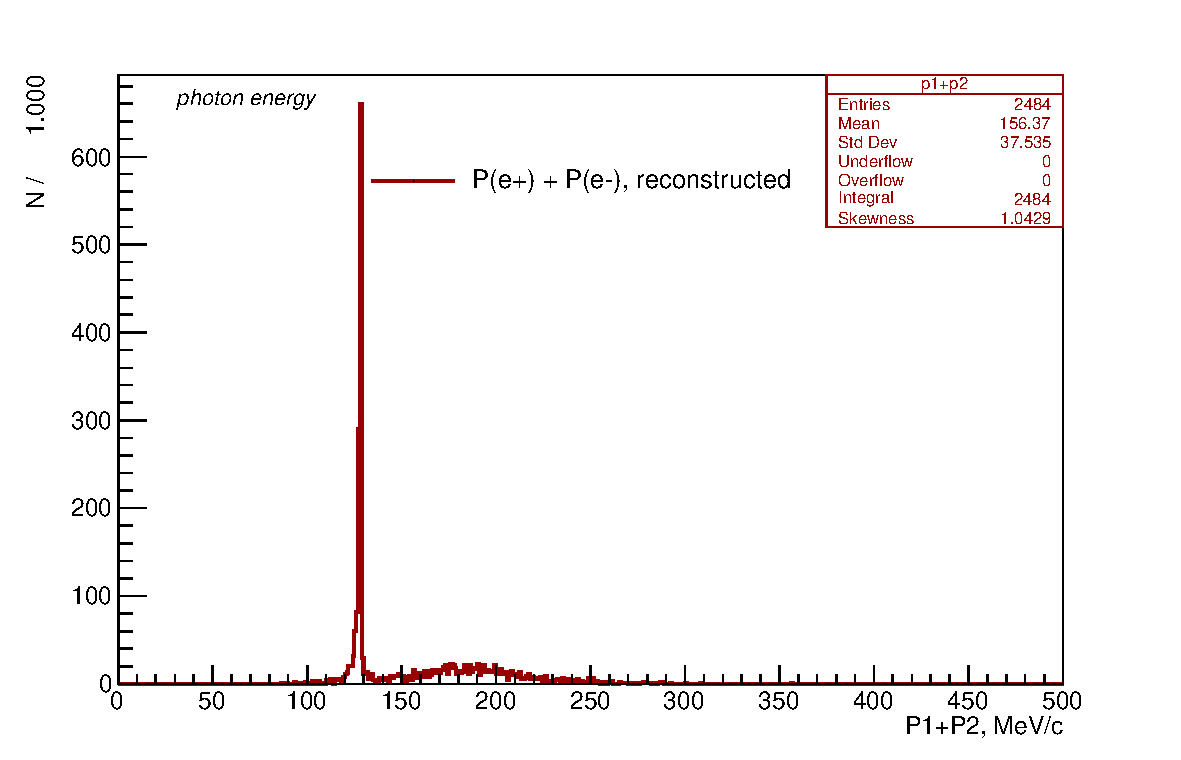
\includegraphics[width=0.95\textwidth]{pdf/figure_00084}
      }
    };
    % \node [text width=8cm, scale=1.0] at (14.5,0.5) {$\mu_B$, expected background mean};
    % \node [text width=8cm, scale=1.0, rotate={90}] at (1.5,7.5) { $S_{D}$, ``discovery'' signal strength  };
  \end{tikzpicture}
  \caption{
    \label{figure:00084_rpc04b0s54_t2_1_smom_0}
    Sum of the two reconstructed track momenta
  }
\end{figure}

Comparison of Figure ~\ref{figure:00084_rpc04b0s54_t2_1_smom_0} 
to Figure ~\ref{figure:00083} gives an estimate of the reconstruction efficiency
for preselected events of about 10\%, which is not very high.
%
However the Mu2e track reconstruction, first of all - the pattern recognition,
has never been tuned for low momentum tracks. An example of a $\gamma \to e^+e^-$
event with two potentially reconstructable, but only one reconstructed track
is shown in Figure ~\ref{figure:event_display}. In this event, there are two particles,
an electron and a positron entering the tracker with the momenta of 83.7 and 43.5 MeV/c
respectively. A particle with the higher momentum, a 83.7 MeV/c electron, has a reconstructed track,
however the positron track has not been found.  

\begin{figure}[H]
  \begin{tikzpicture}
    \node[anchor=south west,inner sep=0] at (0,0.) {
      % \node[shift={(0 cm,0.cm)},inner sep=0,rotate={90}] at (0,0) {}
      \makebox[\textwidth][c] {
        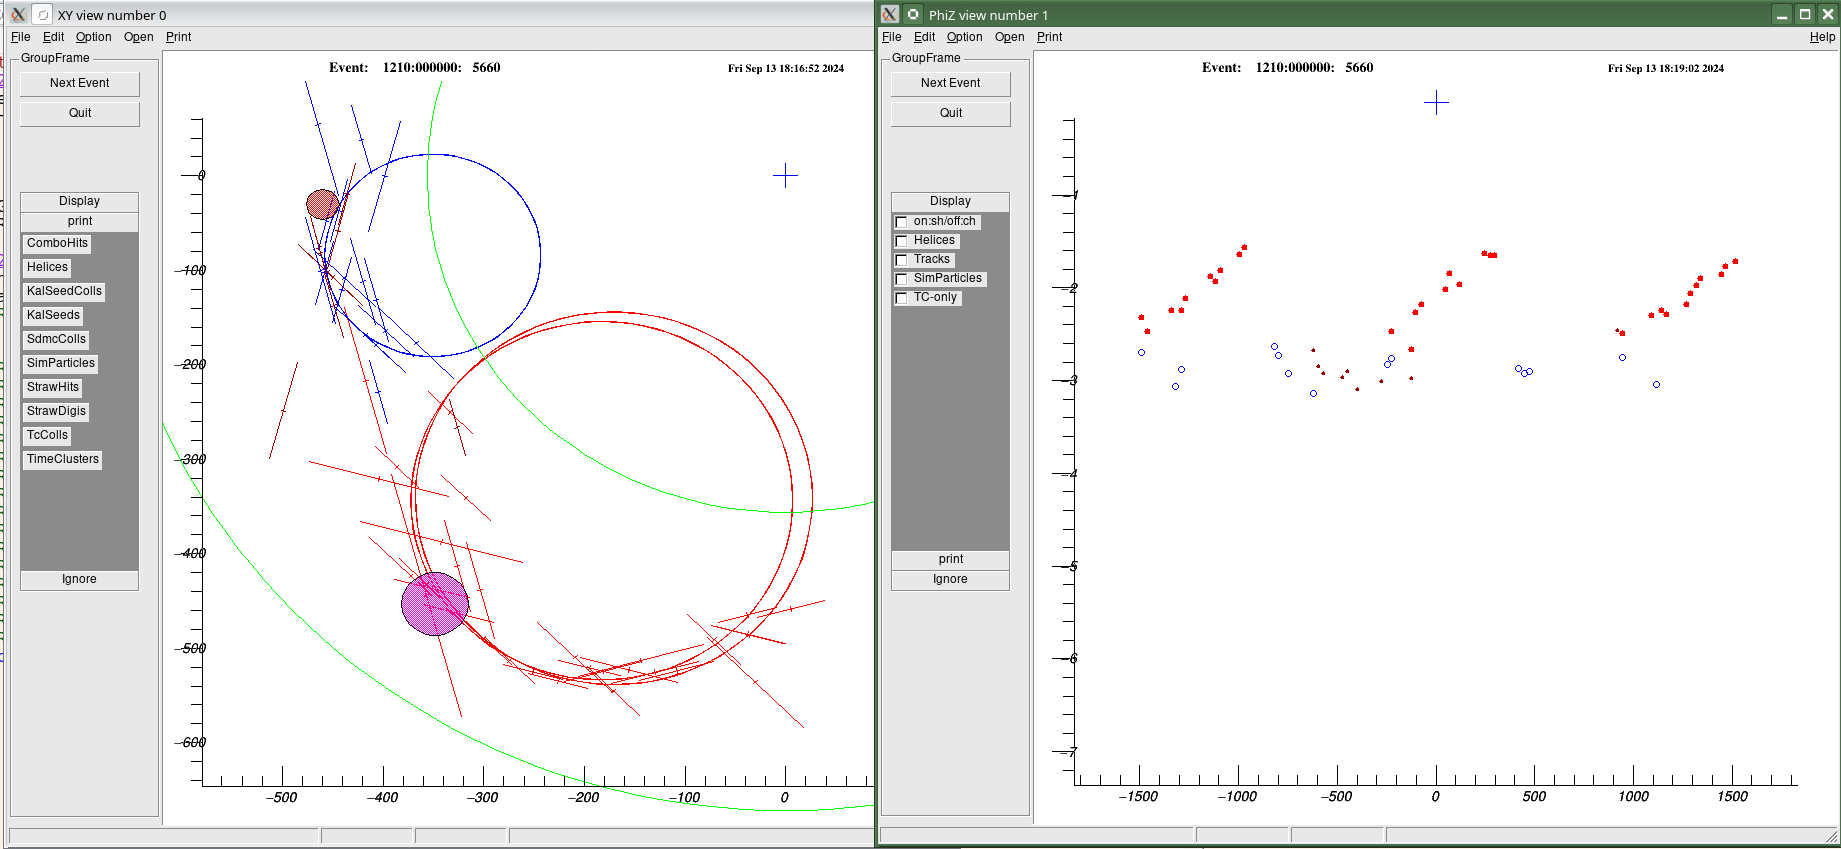
\includegraphics[width=0.95\textwidth]{png/rpc04b0s54r0100_1210_0_005660}
      }
    };
    % \node [text width=8cm, scale=1.0] at (14.5,0.5) {$\mu_B$, expected background mean};
    % \node [text width=8cm, scale=1.0, rotate={90}] at (1.5,7.5) { $S_{D}$, ``discovery'' signal strength  };
  \end{tikzpicture}
  \caption{
    \label{figure:event_display}
    An example of a 129.4 MeV photon conversion event with two tracks
    in the tracker fiducial and only one track (red circle of a smaller radius)
    reconstructed. Shown are the XY and $\phi$-Z event views in the tracker.
    {\red check if some of the positron hits been lost to the delta-electron removal}
  }
\end{figure}

A second type of misreconstruction occurs when hits from both
particles are combined to make an unrealistic track with larger radius
than either true track. These can occur in place of reconstruction for
an individual particle, or in addition to well-reconstructed
tracks. Figure~\ref{figure:he_artifact_evts} shows two
examples. Taking the sum of momenta for cases with one or more of
these combined tracks can significantly overestimate the true total
momentum, and results in high energy artifacts out beyond the original
RPC photon energy. As part of track reconstruction improvements,
better separation of hits between the two tracks will be needed to
recover some of these events.

\begin{figure}[H]
  \begin{tikzpicture}
    \node[anchor=south west,inner sep=0] at (0,0.) {
        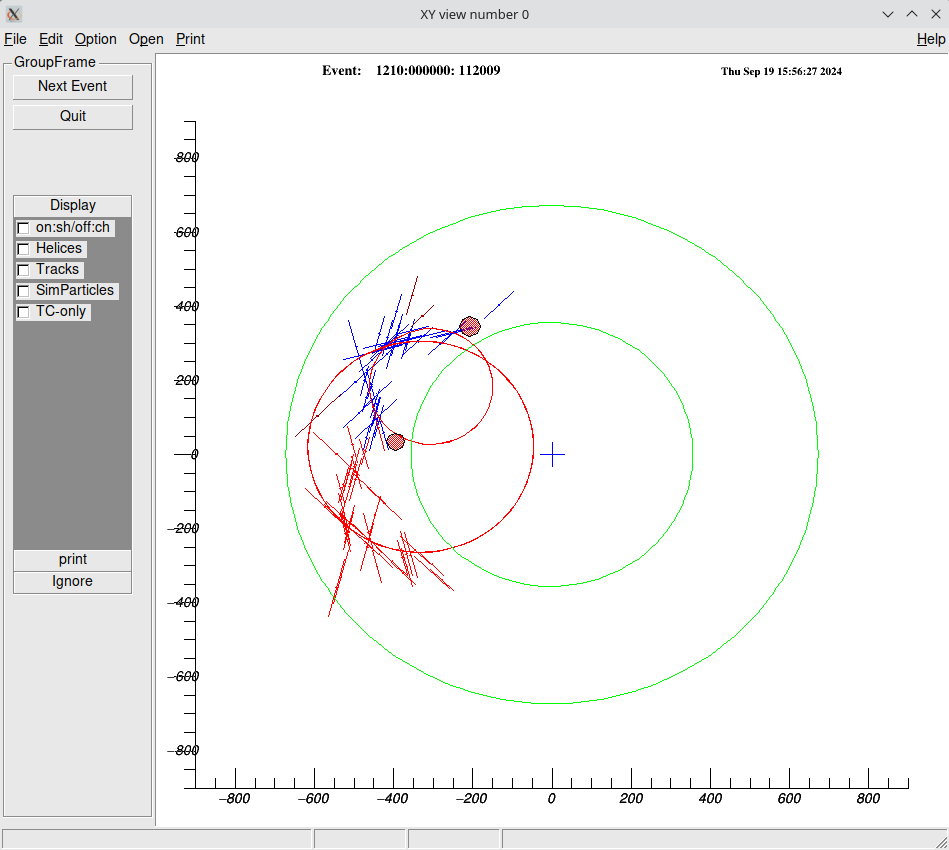
\includegraphics[width=0.54\textwidth]{png/rpc04b0s54r0100_1210_0_112009}
    };
    \node[anchor=south west,inner sep=0] at (9.8,0.) {
        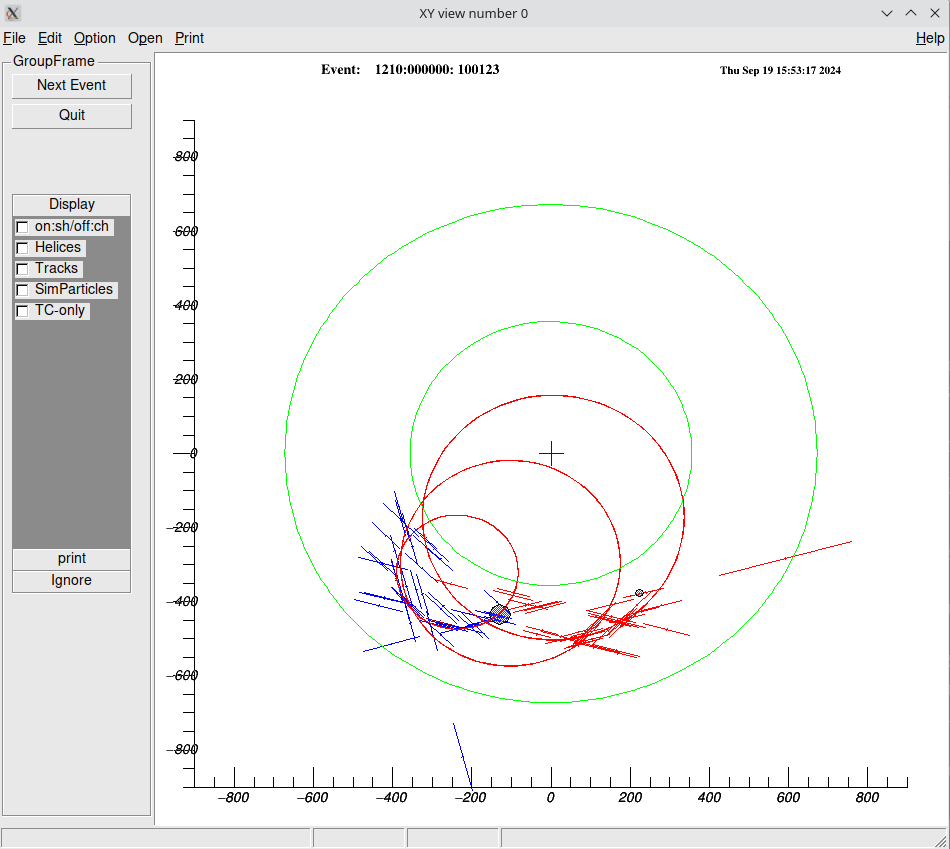
\includegraphics[width=0.54\textwidth]{png/rpc04b0s54r0100_1210_0_100123}
    };
  \end{tikzpicture}
  \caption{
    \label{figure:he_artifact_evts}
    Tracker XY view for two example events where the existing
    reconstruction combines hits from both electron and positron to
    make tracks with unrealistic large transverse momentum. Circles
    include all reconstructed tracks for these events, both artifacts
    and well-reconstructed tracks (no MC truth tracks are shown here).
  }
\end{figure}

Figure~\ref{figure:00085_t2_1_smom_1_fit} shows the fit of the
reconstructed $\pi^- p \to n \gamma$ peak with the SU2020 resolution function.
The peak has its maximum at 128.4 MeV, about 200 keV below the fit
of the MC truth distribution in Figure~\ref{figure:00083},
and the peak width is about 1 MeV FWHM. 

\begin{figure}[H]
  \begin{tikzpicture}
    \node[anchor=south west,inner sep=0] at (0,0.) {
      % \node[shift={(0 cm,0.cm)},inner sep=0,rotate={90}] at (0,0) {}
      \makebox[\textwidth][c] {
        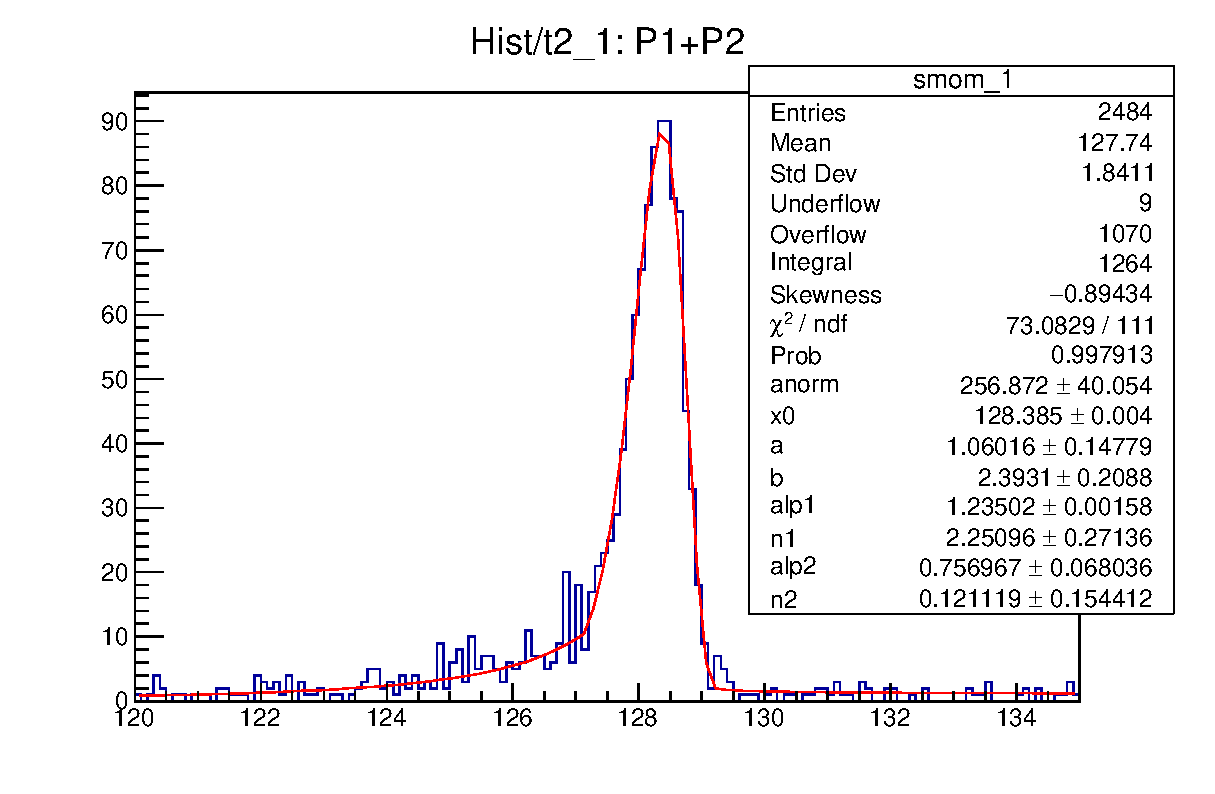
\includegraphics[width=0.95\textwidth]{pdf/figure_00085}
      }
    };
    % \node [text width=8cm, scale=1.0] at (14.5,0.5) {$\mu_B$, expected background mean};
    % \node [text width=8cm, scale=1.0, rotate={90}] at (1.5,7.5) { $S_{D}$, ``discovery'' signal strength  };
  \end{tikzpicture}
  \caption{
    \label{figure:00085_t2_1_smom_1_fit}
    fit of the $\pi^- p \to n \gamma$ peak with the SU2020 resolution function
    in the range [120,135] MeV
  }
\end{figure}

%%% Local Variables:
%%% mode: latex
%%% TeX-master: t
%%% End:
